La fase di Data integration è stata impostata in modo tale da produrre un dataset pulito e direttaemnte sottoponibile ad un modello di Machine Learning.

Gli attributi relativi ai nomi degli atleti, resi necessari dalla mancanza di un ID univoco, vengono rimossi dopo aver effettuato l'integrazione.

\section{Analisi esplorativa}

\par
Il dataset integrato risultante possiede per ciascuno dei 128 000 tiri informazioni relative al tiro e dati relativi agli atleti coinvolti nello scontro che ha portato allo stesso.
\par

In Shot logs sono stati esclusi alcuni attributi (descritti nella \autoref{tabella_shot_logs}) riguardanti la partita come \texttt{W}, \texttt{Final margin} e \texttt{Matchup}, ritenuti non rilevanti per le sorti di un tiro a canestro.
Anche \texttt{Period} e \texttt{Game clock} sono stati ritenuti superflui, in quanto è già presente l'attributo \texttt{Shot number}, così come non significativo è stato valutato l'attributo \texttt{Pts type} (deducibile dall'attributo \texttt{Shot distance}). 
\par
Analogamente, in Seasons stats sono stati esclusi decine di indici statistici non determinanti, oltre agli attributi (descritti in \autoref{tabella_seasons_stats}) come \texttt{Games} e \texttt{MP}.

\par

Alcuni dati che sarebbe stato interessante avere, ma assenti nelle nostri fonti, riguardano informazioni più specifiche inerenti alla partita, come ad esempio la precisa posizione dei giocatori sul rettangolo di gioco piuttosto che l’effettiva distanza tra essi, oppure la stabilità dell’attaccante durante il tiro (o durante la difesa nel caso del difensore). Queste e altre dinamiche di gioco permetterebbero di creare modelli più approfonditi in modo da fornire predizioni più fedeli.

\par
I valori da predire sono distribuiti in modo non uniforme. Il 55\% (70157 record) sono tiri \textit{missed}, mentre il 45\% (57900 record) sono tiri \textit{made}(\autoref{dist_shot_result}).

\begin{figure}
\caption{Distribuzione degli esiti nel dataset integrato}
\label{dist_shot_result}
	\includegraphics[width=\linewidth]{shot_result}
\end{figure}

\par

\begin{figure}
\caption{Importanza delle feature, secondo il modello prodotto}
\label{importance_fig}
\fontsize{9pt}{1em}
	\includegraphics[width=\linewidth]{importance}
\end{figure}

\par

\textit{Importance}, mostrata nella \autoref{importance_fig}, rappresenta il contributo informativo delle feature considerate. Le principali risultano \texttt{shot\_dist}, \texttt{close\_def\_distance} e \texttt{dribbles}.

\begin{figure}
\caption{Correlazione tra gli attributi più rilevanti}
\label{plot_shot_dist_def}
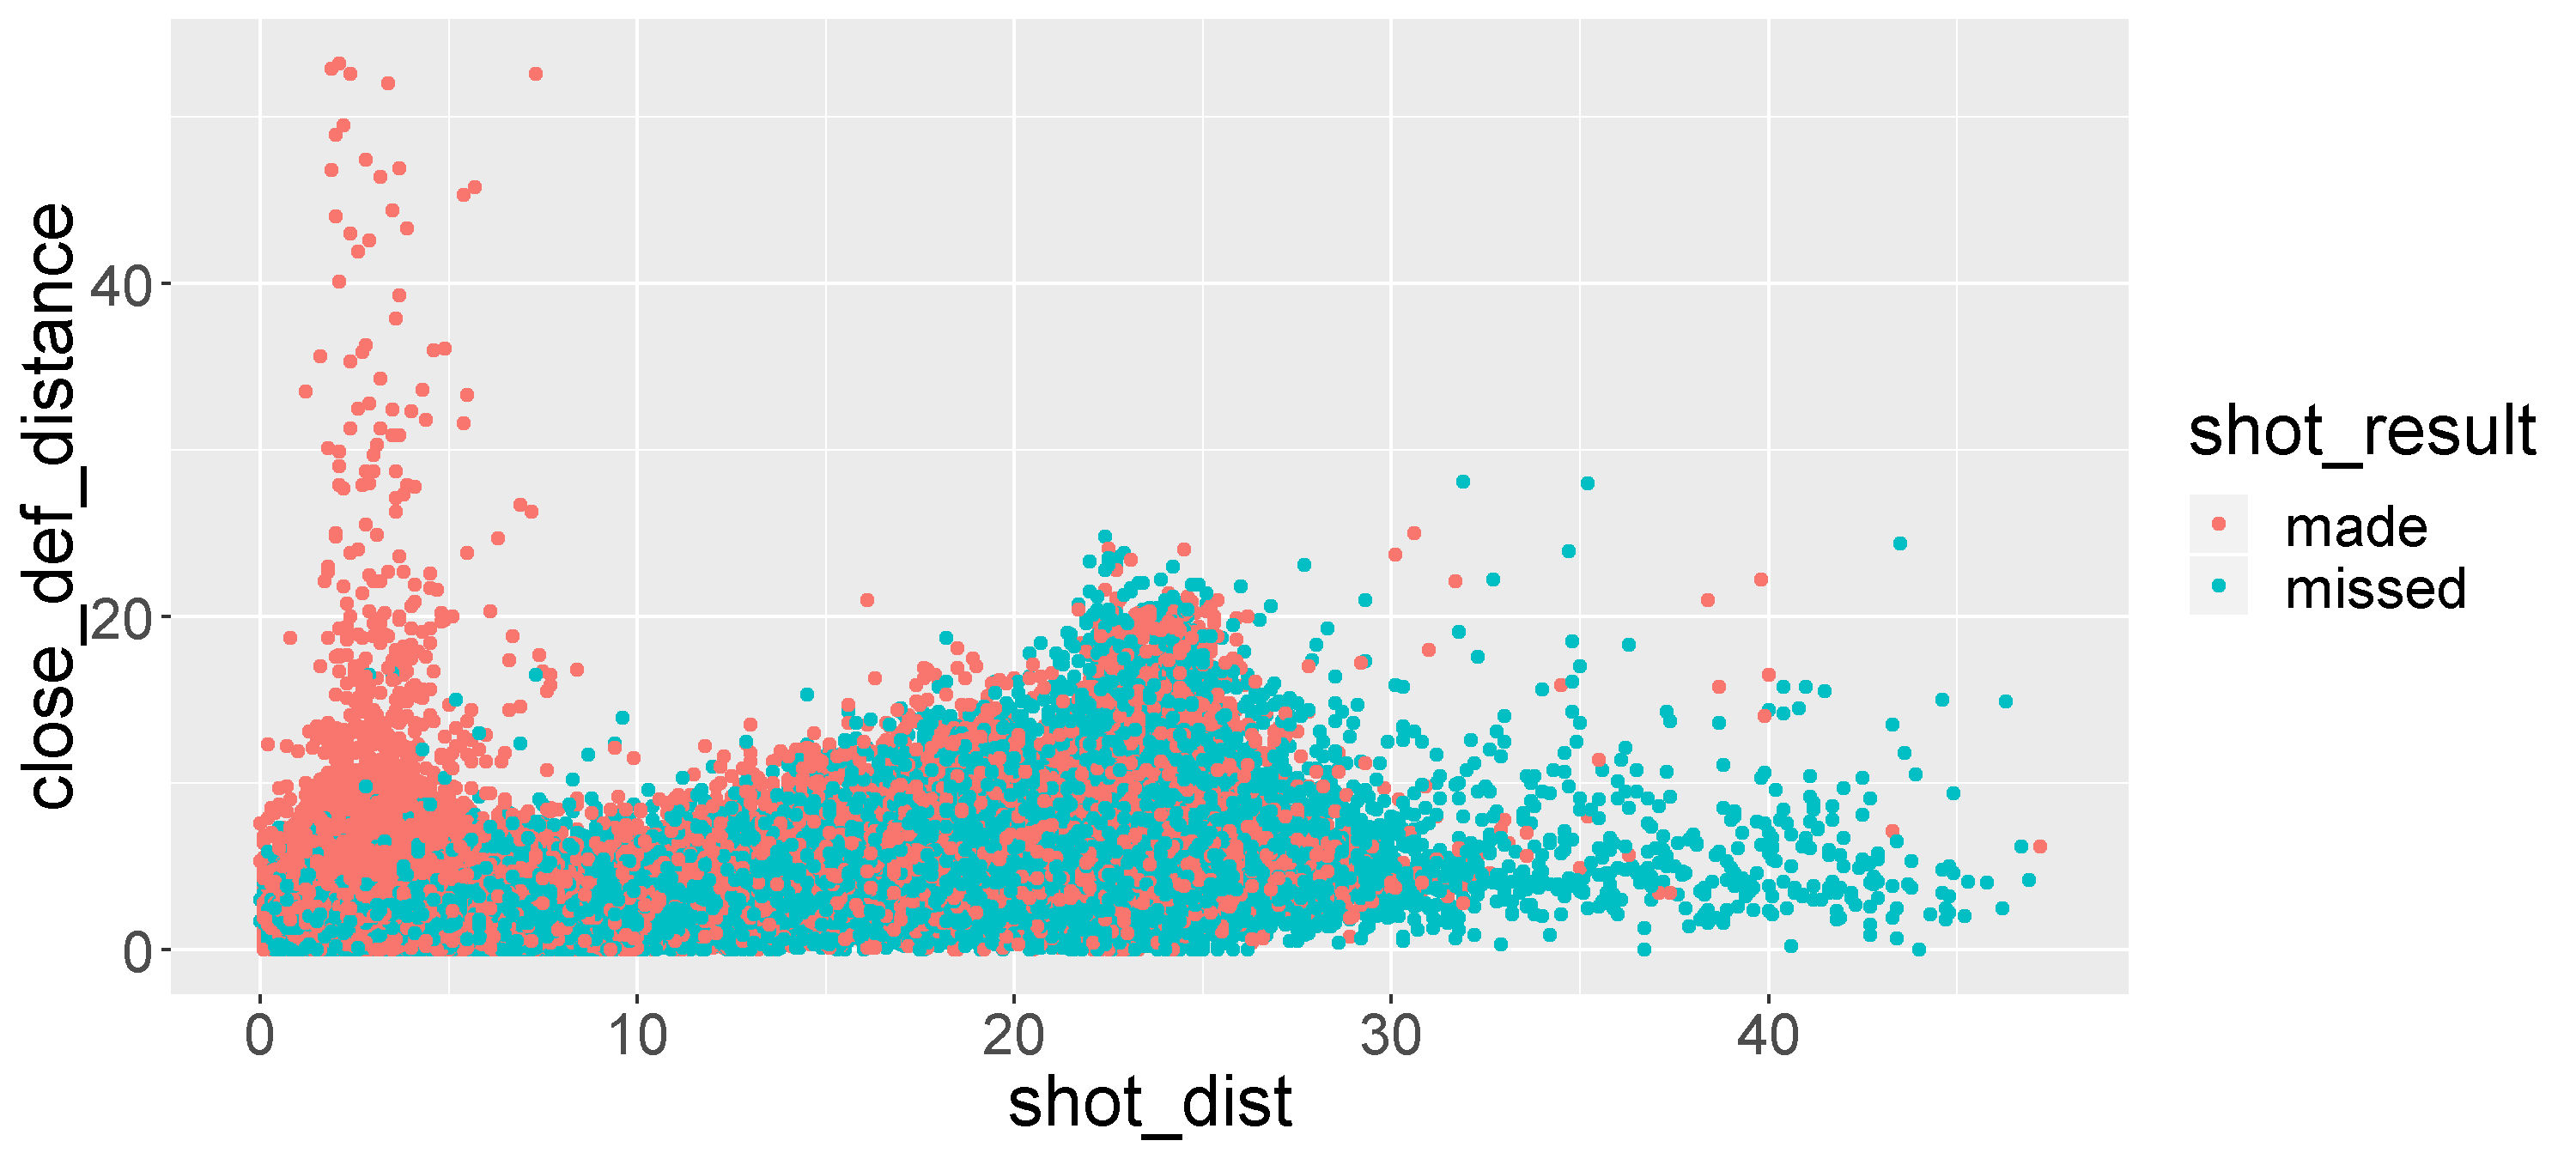
\includegraphics[width=\linewidth]{plot_shot_dist_def.png}
\end{figure}

Il grafico è stato interpretato considerando due regioni: la regione con prevalenza \texttt{made}, ossia quella compresa tra $[0, 10]$ nell'asse delle ascisse e $[5, 40+] $ nell'asse delle ordinate, e la regione con prevalenza \texttt{missed}, ossia quella compresa tra $[25, 40]$ nell'asse delle ascisse e $[0, 20] $ nell'asse delle ordinate.
Abbiamo intepretato le distribuzioni di queste due regioni rintracciando quello che succede sul campo: i tiri effettuati dal pitturato (area sottostante al canestro), seppur con il difensore alle calcagne, hanno una probabilità di essere messi a segno molto alta. I tiri effettuati dalla distanza, invece, sono di notevole difficoltà e la probabilità di fallimento è alta anche se l'attaccante è un giocatore efficiente ed affidabile.

\par

\begin{figure}
\caption{Distanza media del tiro rispetto al ruolo del giocatore}
\label{position_shot_dist}
\includegraphics[width=\linewidth]{shot_dist_with_position}
\end{figure}

Il grafico in \autoref{position_shot_dist} mostra che C, il componente della squadra che domina il pitturato, tira in media da una distanza inferiore ai 10 piedi, seguito da PF. I giocatori in questo ruolo prendono quindi tiri meno rischiosi.
Non abbiamo a disposizione informazioni relative a peso e altezza, ma i dati  \cite{basketball-reference} mostrano che in media in questi due ruoli giocano gli atleti più fisicamente dotati: soffrendo meno il contatto con l'avversario riescono a raggiungere più facilmente il canestro.

Al contrario, gli altri tre ruoli (PG, SF e SF) tirano da una distanza che si aggira intorno ai 15 piedi. Sono meno prestanti dal punto di vista fisico ma solitamente con un'abilità al tiro maggiore, che li porta a prendere anche tiri rischiosi e più difficili, portando ad abbassare le loro statistiche.

\begin{figure}
\caption{Successo dei tiri rispetto al ruolo del giocatore}
\label{position_shots}
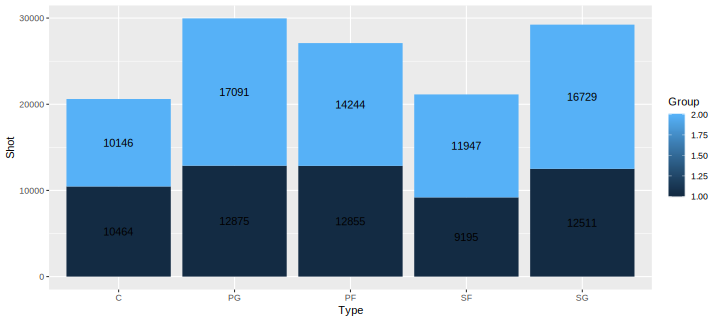
\includegraphics[width=\linewidth]{made_missed_barplot}
\end{figure}

La \autoref{position_shots} conferma questa intepretazione: PF ha una percentuale di missed pari a 0.53; ancora più bassa la percentuale di missed per C, pari a 0.49: l'unico ruolo ad avere un numero di tiri made maggiori rispetto ai missed ma anche la posizione con il numero minore di tiri effettuati.

I tre ruoli più delicati (PG, SF, SG) hanno una percentuale di missed pari a 0.57.